\section{Analysis Metric 3: Longest Line Length}
\label{sec:analysisLLL}

The third metric we analyzed is the length of the longest line found across all plain-text files of an \ac{NPM} package version, 
expressed in number of characters.
It was motivated by the observation that Attacks~B (\cref{sec:attackB}),
C (\cref{sec:attackC}), and D (\cref{sec:attackD}) all inject malicious code formatted as a single, extremely long line.
Specifically, Attack~B adds 76,438 characters to an existing \texttt{index.js},
while Attacks~C and D introduce files containing lines of 3,734,355 and 10,157,373 characters, respectively.
The intuition is that legitimate packages rarely contain code with lines of such extreme length, making this an anomalous signal.
To verify this, we first characterized the distribution of this metric in the \emph{Goodware} dataset,
paying particular attention to the role of build artifacts, 
automatically generated files that can also produce long lines, 
and then evaluated whether the malicious releases deviate detectably from that baseline.

\subsection{Analysis of the Goodware Dataset}
\label{subsec:goodwareLLL}

\begin{figure}[htbp]
    \centering
    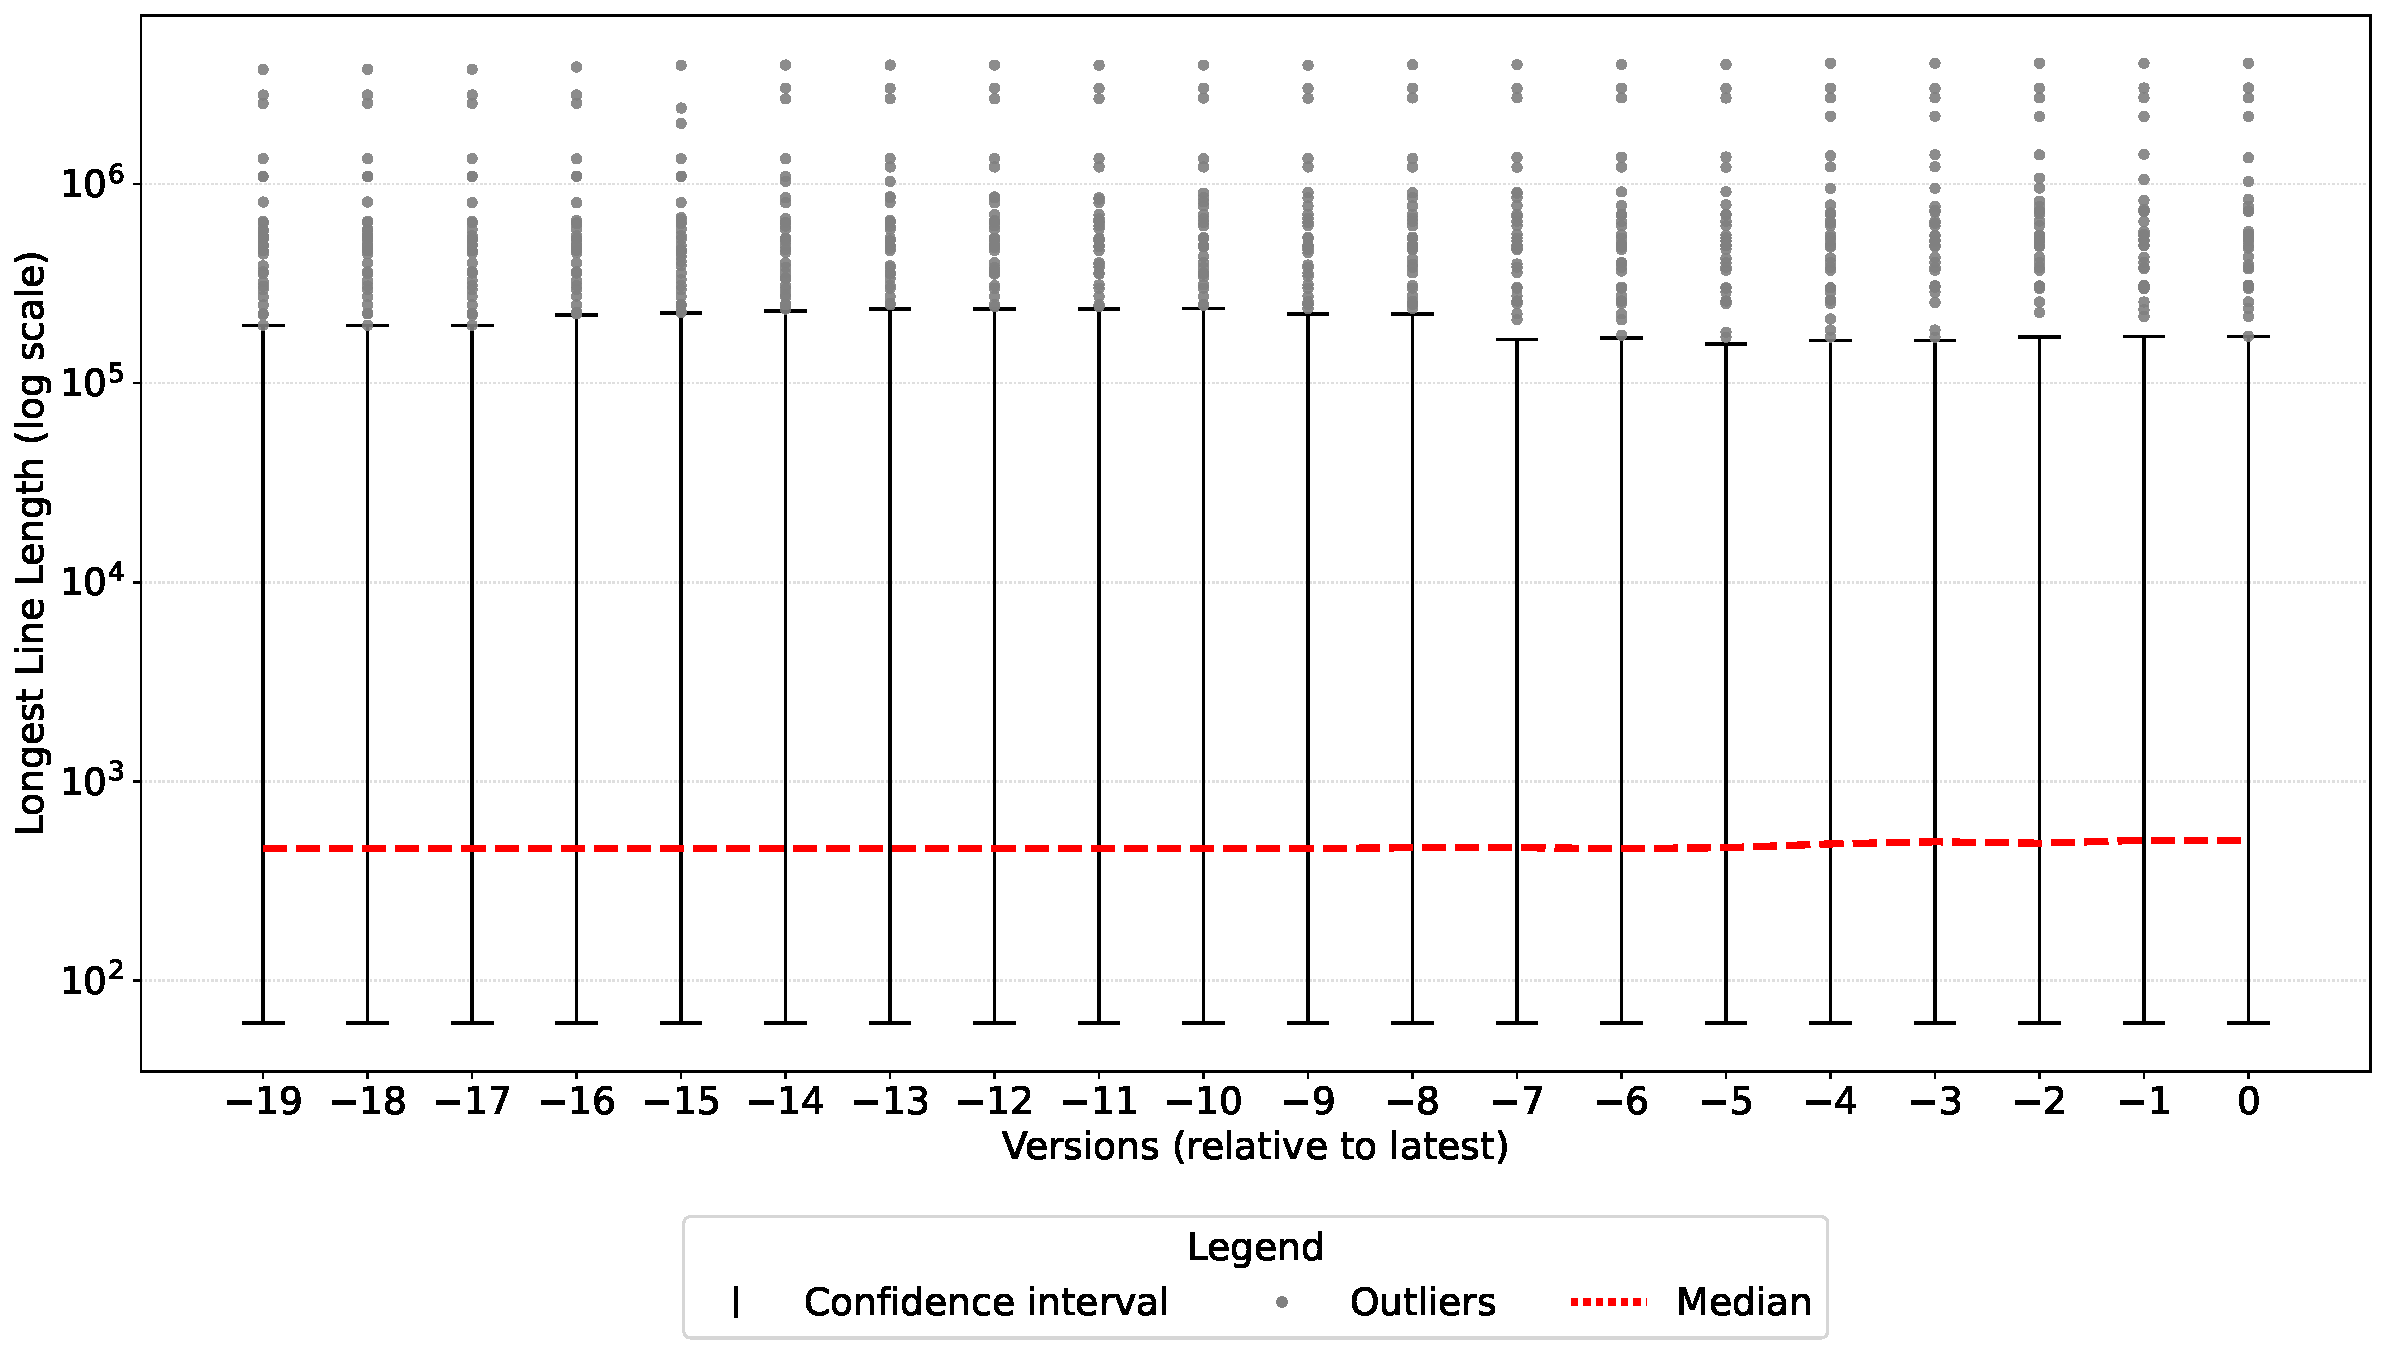
\includegraphics[width=\textwidth]{metrics/LongestLineLength/LLL_plot1.pdf}
    \caption{Longest Line Length Metric: Package Trend in Goodware Dataset.}
    \label{fig:fig1LLL}
\end{figure}

The \emph{Goodware} dataset provides, for each of the 629 packages,
the longest line length observed across all plain-text files in their 20 analyzed versions,
as described in \cref{subsec:goodwareDataset}.
To visualize the distribution and evolutionary patterns of this metric across releases,
we used \cref{fig:fig1LLL,fig:fig1LLLTrend}; 
where we can observe that the median remains stable at approximately 460 characters, 
indicating that the length of the longest line does not change significantly in the typical package.
This stability is a useful property for anomaly detection, 
as a sudden large increase is precisely the signature left by the \acp{SSCA} considered.

An important caveat is that build artifacts, 
such as source map files (\texttt{.map}) and compiler-generated JavaScript, 
can legitimately contain very long lines, and are therefore a potential source of false positives for this metric.
In this analysis, we chose to include the entire tarball contents without excluding any file type or directory a priori,
because an attacker could inject malicious code anywhere within the tarball.

\begin{figure}[htbp]
    \centering
    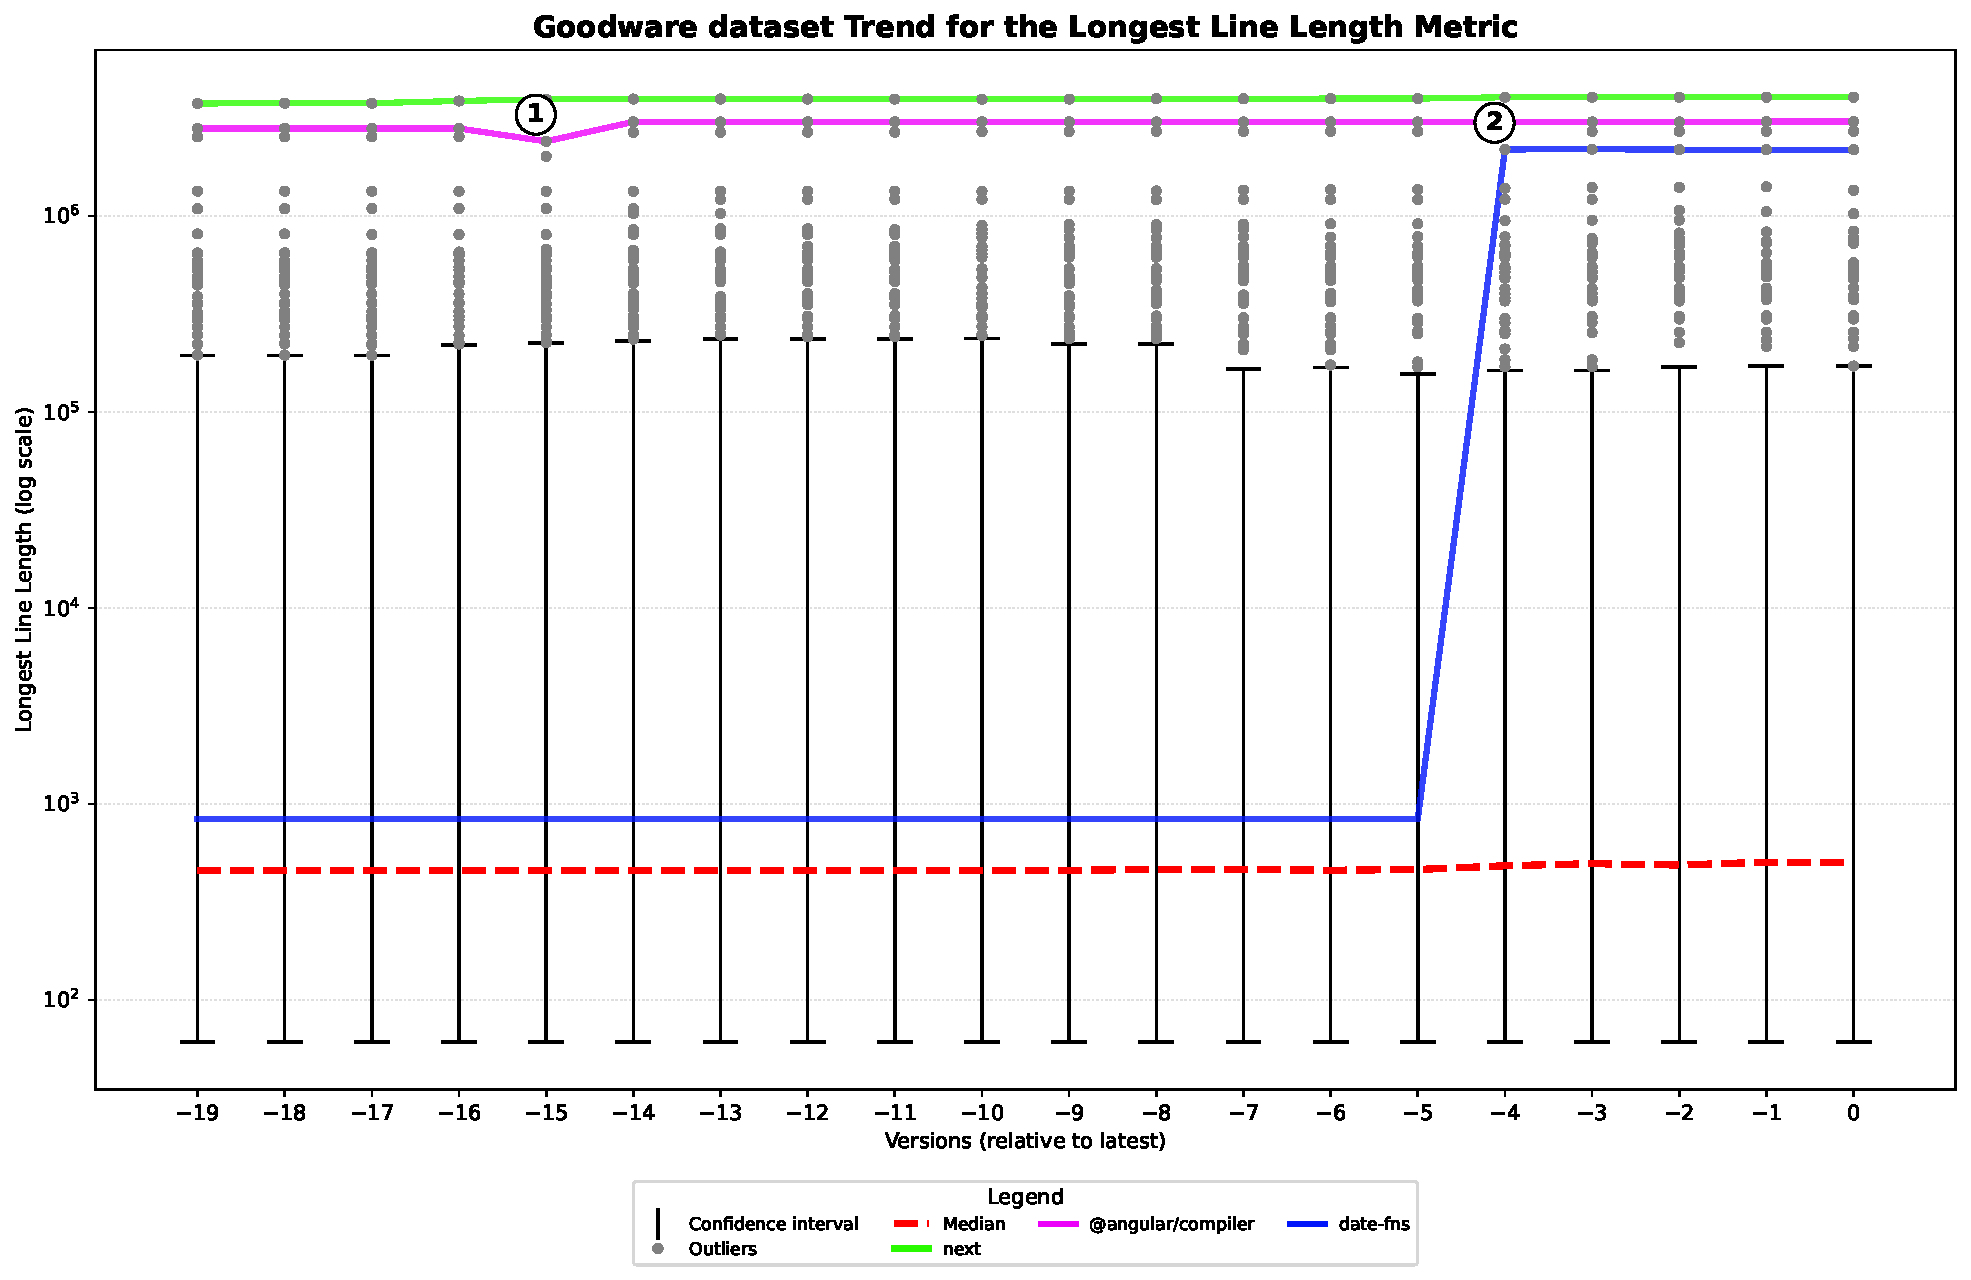
\includegraphics[width=\textwidth]{metrics/LongestLineLength/LLL_plot1_Trend.pdf}
    \caption{Longest Line Length Metric: Outliers Package Trend in Goodware Dataset.}
    \label{fig:fig1LLLTrend}
\end{figure}

As shown in \cref{fig:fig1LLLTrend}, 
from the \emph{Goodware} dataset we selected three packages for individual analysis as representative cases, 
as they exhibit outlier values directly attributable to build artifacts.

\textbf{next} (solid green line) is a React full-stack framework~\cite{next}.
It shows the most extreme outlier in the entire \emph{Goodware} dataset, 
with a longest line length of 4,041,545 characters, present in all 20 versions.
This value originates from the file \texttt{app-page-turbo-\allowbreak experimental.runtime.dev.js.map},
a source map file consisting of a single line.
The \texttt{next} package also contains other build artifacts with very long lines,
such as \texttt{app-page\allowbreak .runtime.dev.js}, a generated JavaScript file containing 40 lines with the longest reaching 513,963 characters.
Both files are located in the \texttt{dist} folder;
however, it is not guaranteed that build artifacts are always present in any specific directory,
as their location depends entirely on the individual developer choices.

\textbf{@angular/compiler} (solid pink line) is the official compiler of the Angular framework, 
responsible for tasks such as translating templates with Angular syntax~\cite{angular-compiler}.
In all releases, the longest line originates from the file \texttt{compiler.mjs.map} in the \texttt{fesm2022} directory, 
consistently around 3,000,000 characters, making it the second most extreme outlier value in the \emph{Goodware} dataset after \texttt{next}.
As indicated at point~1 in \cref{fig:fig1LLLTrend}, 
in version 21.0.0-rc.0 this value decreased to approximately 2,500,000 characters,
reflecting a natural variation in the output of the build process for that release.
This variability shows that even stable outlier values from build artifacts are not perfectly constant.
\texttt{@angular/compiler} also contains other build artifacts, 
such as \texttt{compiler.mjs}, a generated JavaScript file containing approximately 30,000 lines with the longest reaching 14,825 characters.

\textbf{date-fns} (solid blue line) shows that build artifacts can be introduced in a new release without having been present in previous ones.
Before version 3.6.0, this package was within the confidence intervals, 
but at point~2 in \cref{fig:fig1LLLTrend} the metric jumped to 2,188,784 characters, making it an outlier for all subsequent releases.
This sudden increase was caused by the addition of \texttt{cdn.js.map} in the \texttt{locale} directory, 
consisting of 10 lines with the longest being 2,188,784 characters, making it the longest line found across all plain-text files in the package.
It was introduced in version 3.6.0 together with approximately 400 new files for compatibility with older browsers,
as already discussed in \cref{subsec:goodwarePackageSize}.
The sudden change in this metric is superficially similar to what a malicious injection would produce, 
with the difference that this one is documented~\cite{date-fns_release_notes}.
In this version, \texttt{date-fns} also includes other build artifacts, 
such as the file \texttt{cdn.js} containing 10 lines with the longest being 777,296 characters.

\subsection{Comparison with the Malware Dataset}
\label{subsec:analysisLLLComparisonMalware}

\textbf{Attack~A} (Malicious Windows DLL, \cref{sec:attackA}) includes a plain-text script \texttt{install.js}, 
which, however, does not contain the longest line in the compromised versions; 
and the malicious \ac{DLL} was correctly excluded from the computation, as it is not a plain-text file.
Consequently, the longest line length of the compromised releases remained unchanged compared 
to the preceding legitimate versions, as shown in \cref{fig:fig2LLLAttackA},
making this metric not indicative for this attack.

\textbf{Attack~B} (Crypto attack, \cref{sec:attackB}) adds a single malicious line of 76,438 characters to an existing \texttt{index.js}.
As shown in \cref{fig:fig2LLLAttackB}, this produces a notable increase in the metric,
but not enough to position the compromised releases among the outlier values.
The reason is that the \emph{Goodware} baseline includes packages with build artifacts containing lines of several tens of thousands in length, 
which sets the 95th-percentile bound at approximately 200,000 characters.
The metric is therefore not indicative for this attack.

\textbf{Attack~C} (\texttt{Shai-Hulud}~1.0, \cref{sec:attackC}) introduces a malicious file named \texttt{bundle.js} 
containing a single line of 3,734,355 characters.
As shown in \cref{fig:fig2LLLAttackC}, this places the compromised versions among the outlier values of the \emph{Goodware} distribution.
The metric is therefore effective for detecting Attack~C.

\textbf{Attack~D} (\texttt{Shai-Hulud}~2.0, \cref{sec:attackD}) introduces a malicious file 
\texttt{bun\_environment.js} containing a single line of 10,157,373 characters.
As shown in \cref{fig:fig2LLLAttackD}, the compromised releases not only enter
the outlier range but far exceed the maximum outlier values in the \emph{Goodware} dataset.
The metric is clearly effective for detecting Attack~D.

In summary, despite this metric being influenced by the presence of build artifacts in legitimate packages,
it effectively detects Attacks~C and~D, whose injected files contain a line long enough to exceed the 95th-percentile bound.
Instead, it is not indicative for Attacks~A and~B, since 
the first scenario involves a binary file that is excluded from computation,
while the malicious line of 76,438 characters introduced by Attack~B 
remains within the upper confidence interval bound established in the \emph{Goodware} dataset.

\begin{figure}[htbp]
    \centering
    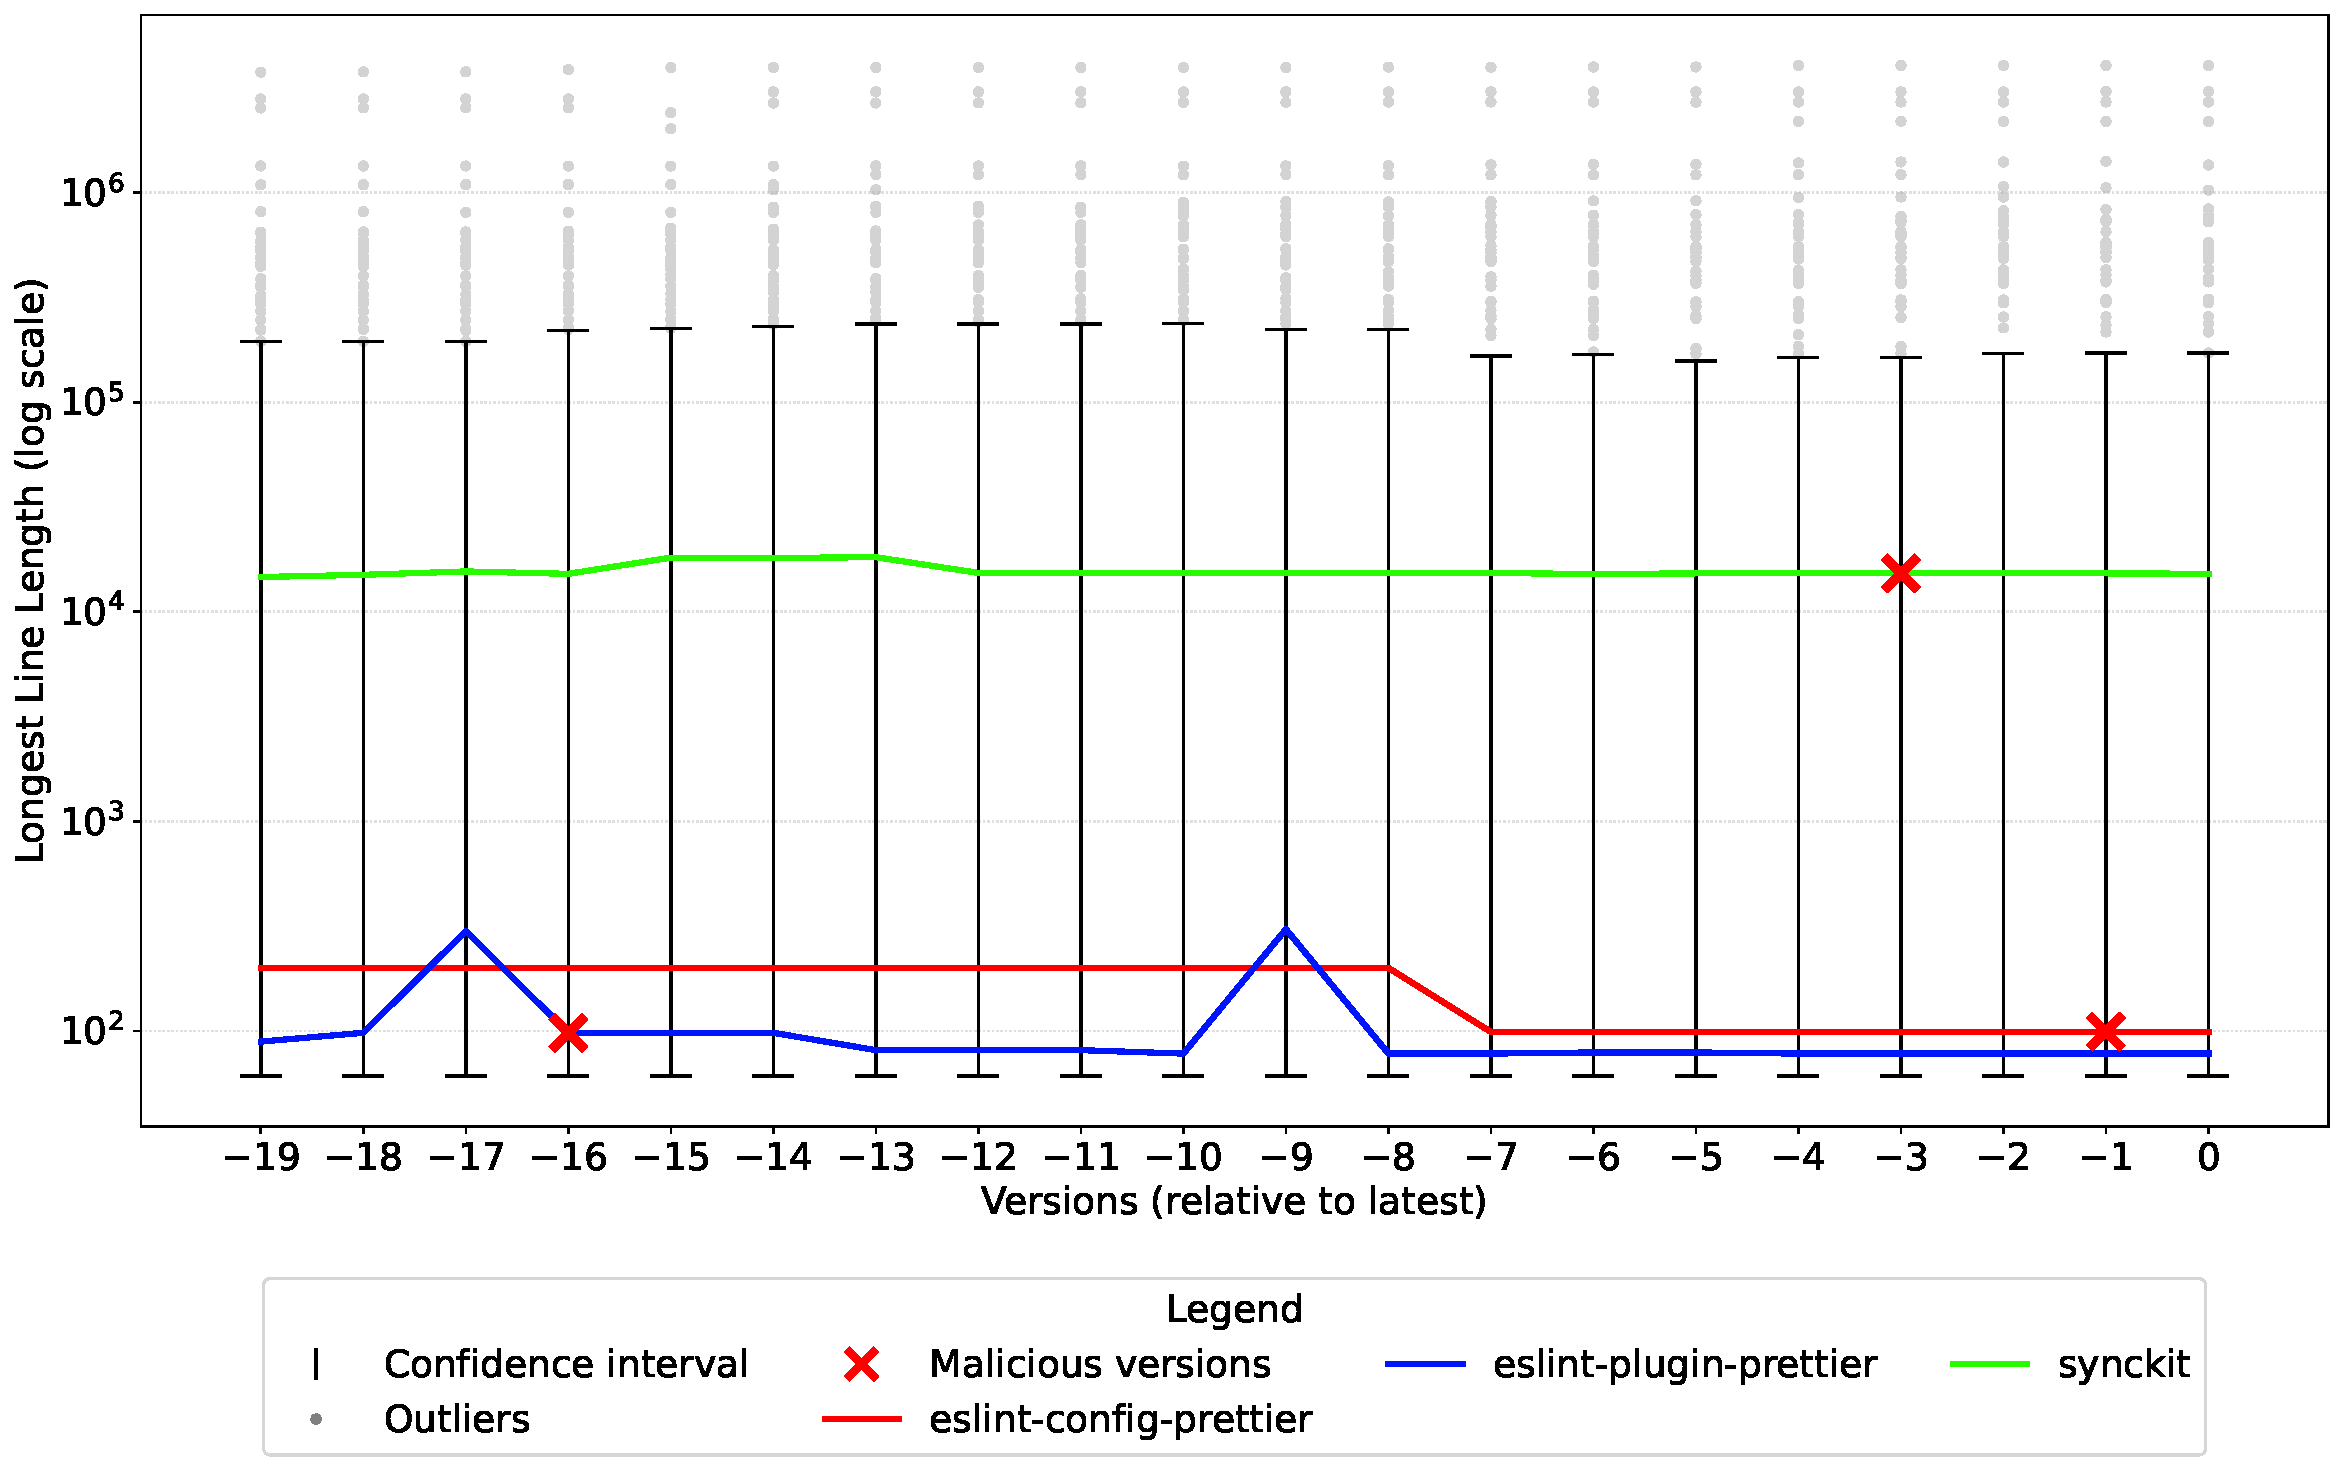
\includegraphics[width=0.90\textwidth]{metrics/LongestLineLength/LLL_plot2single_AttackA.pdf}
    \caption{Longest Line Length Metric: Malware Comparison for Attack~A.}
    \label{fig:fig2LLLAttackA}

    \vspace{0.3cm} % Spazio verticale tra i due grafici
    
    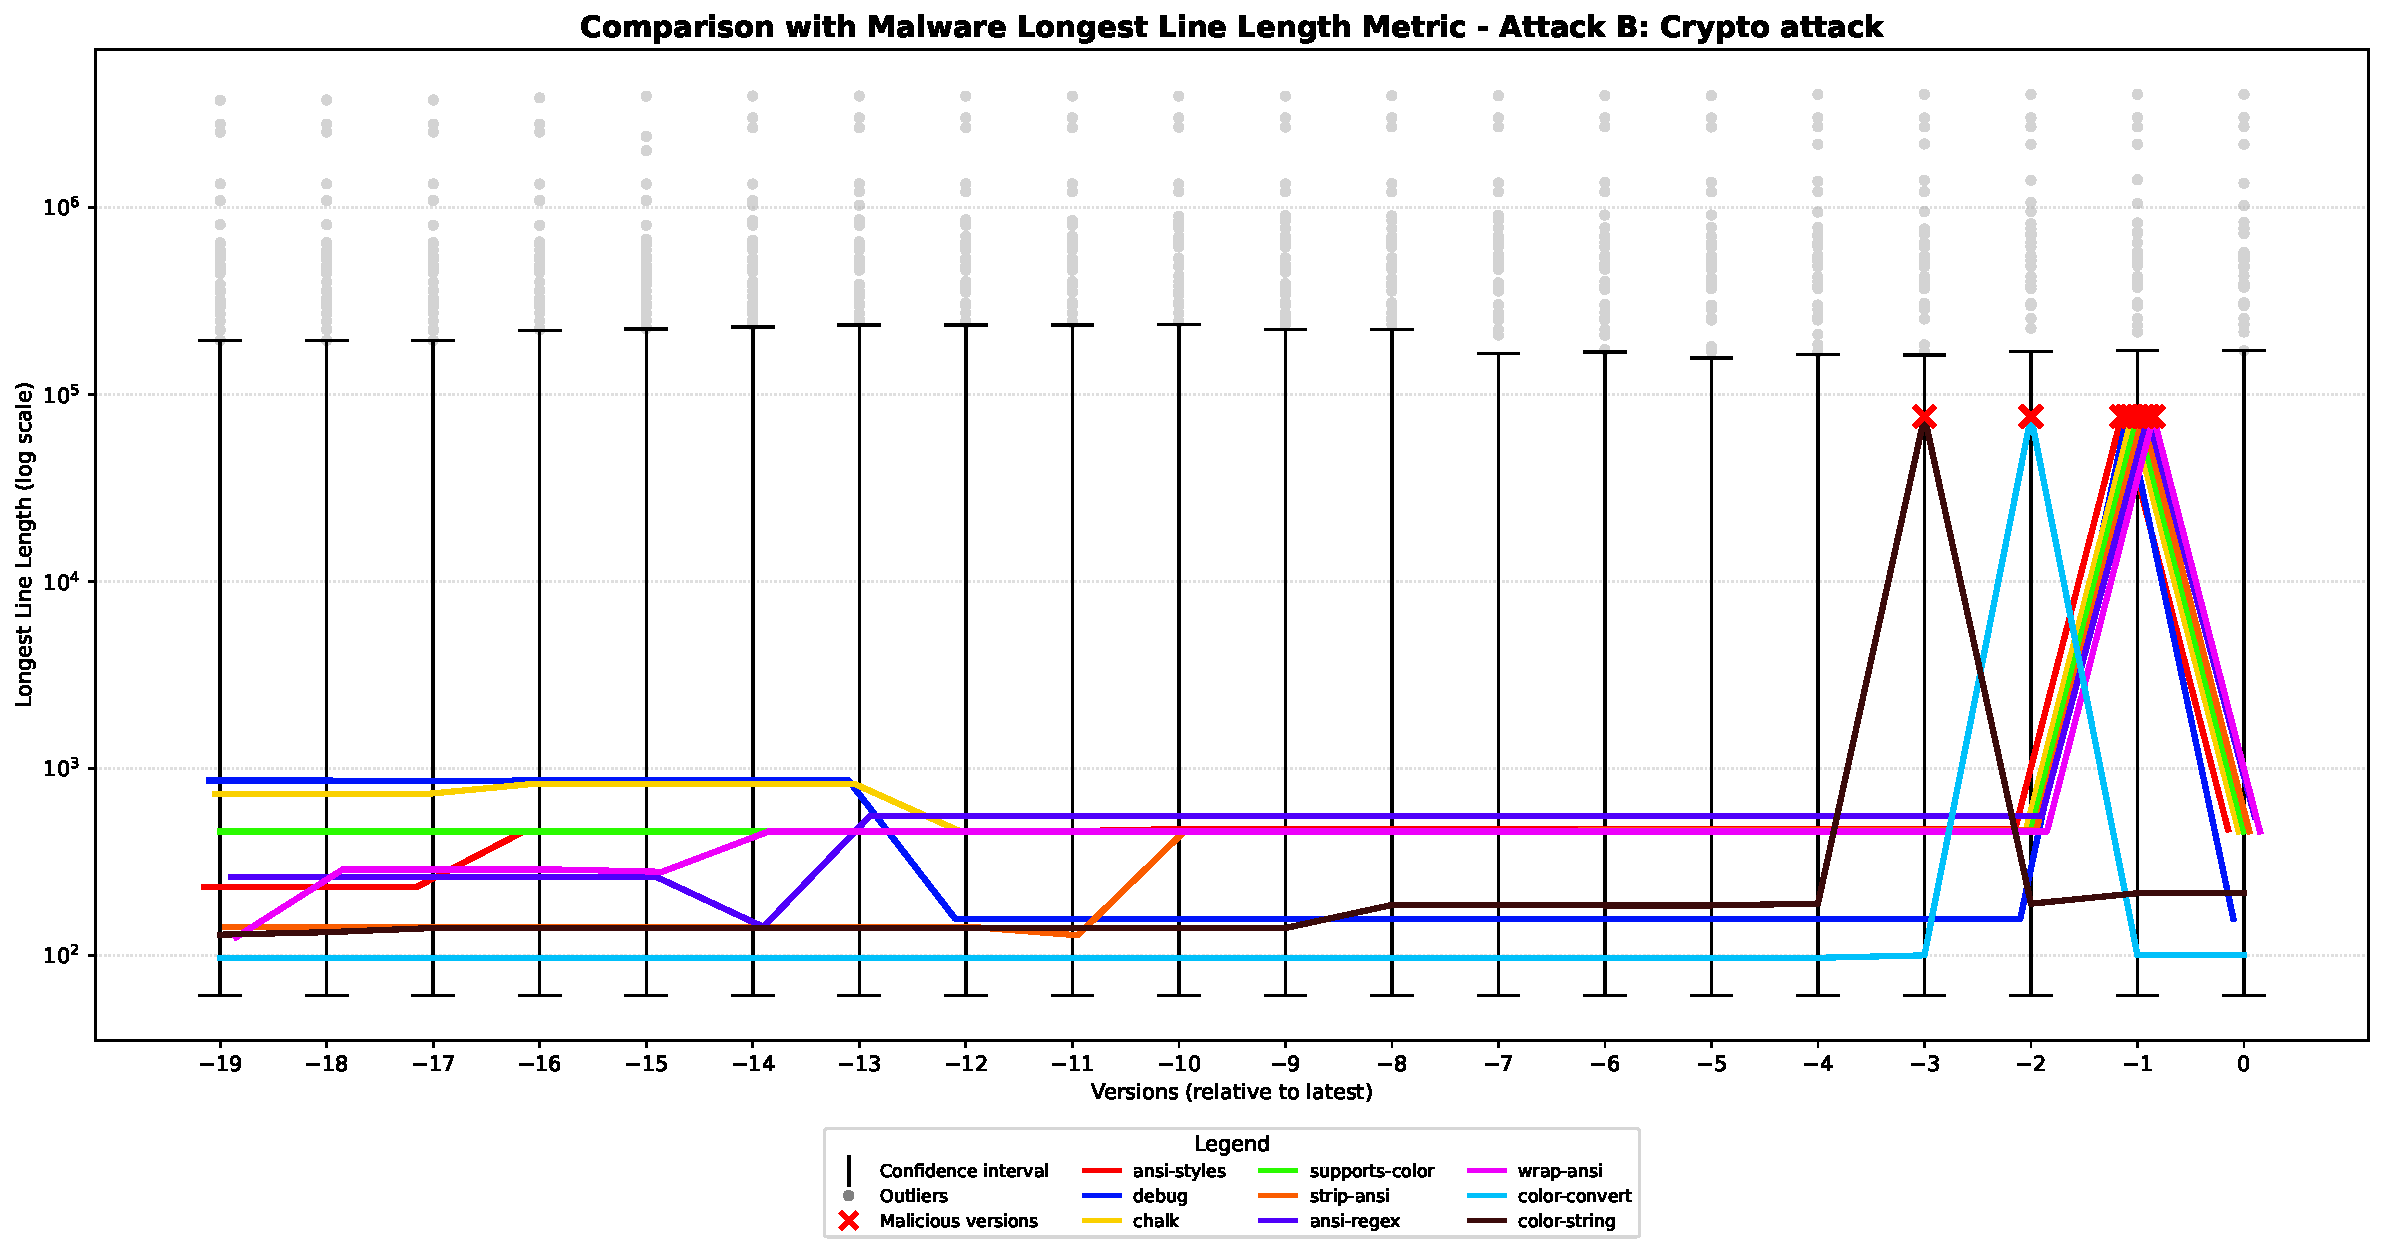
\includegraphics[width=0.90\textwidth]{metrics/LongestLineLength/LLL_plot2single_AttackB.pdf}
    \caption{Longest Line Length Metric: Malware Comparison for Attack~B.}
    \label{fig:fig2LLLAttackB}
\end{figure}

\begin{figure}[htbp]
    \centering
    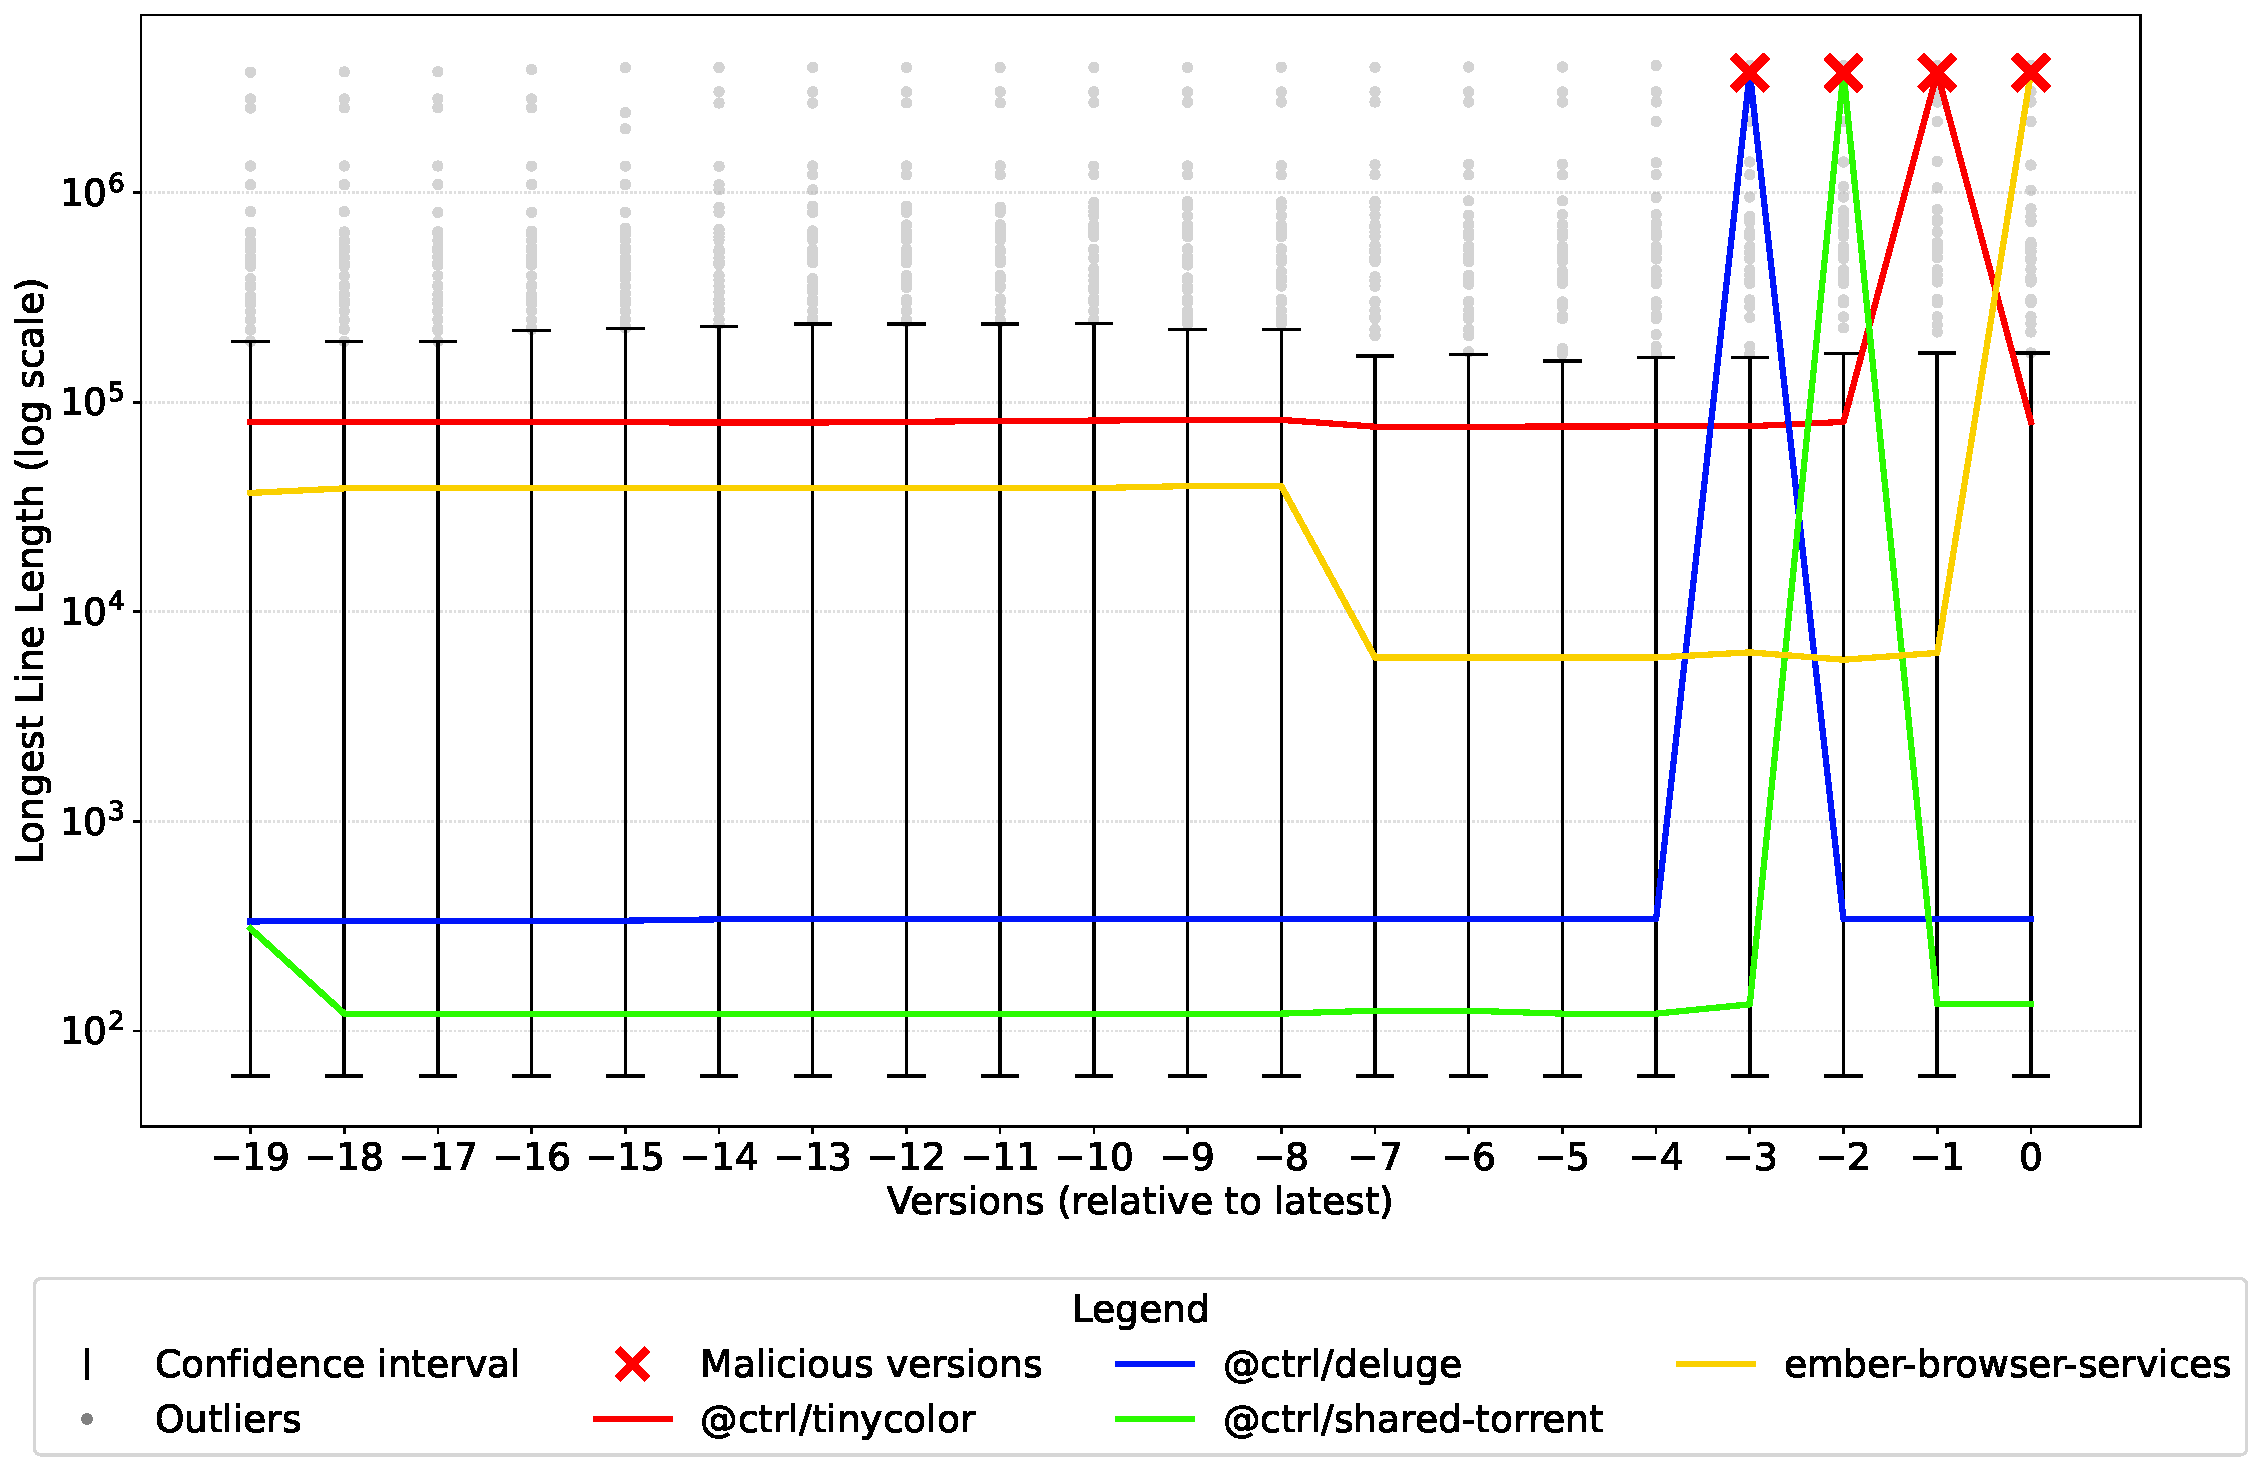
\includegraphics[width=0.90\textwidth]{metrics/LongestLineLength/LLL_plot2single_AttackC.pdf}
    \caption{Longest Line Length Metric: Malware Comparison for Attack~C.}
    \label{fig:fig2LLLAttackC}
    
    \vspace{0.3cm} % Spazio verticale tra i due grafici
    
    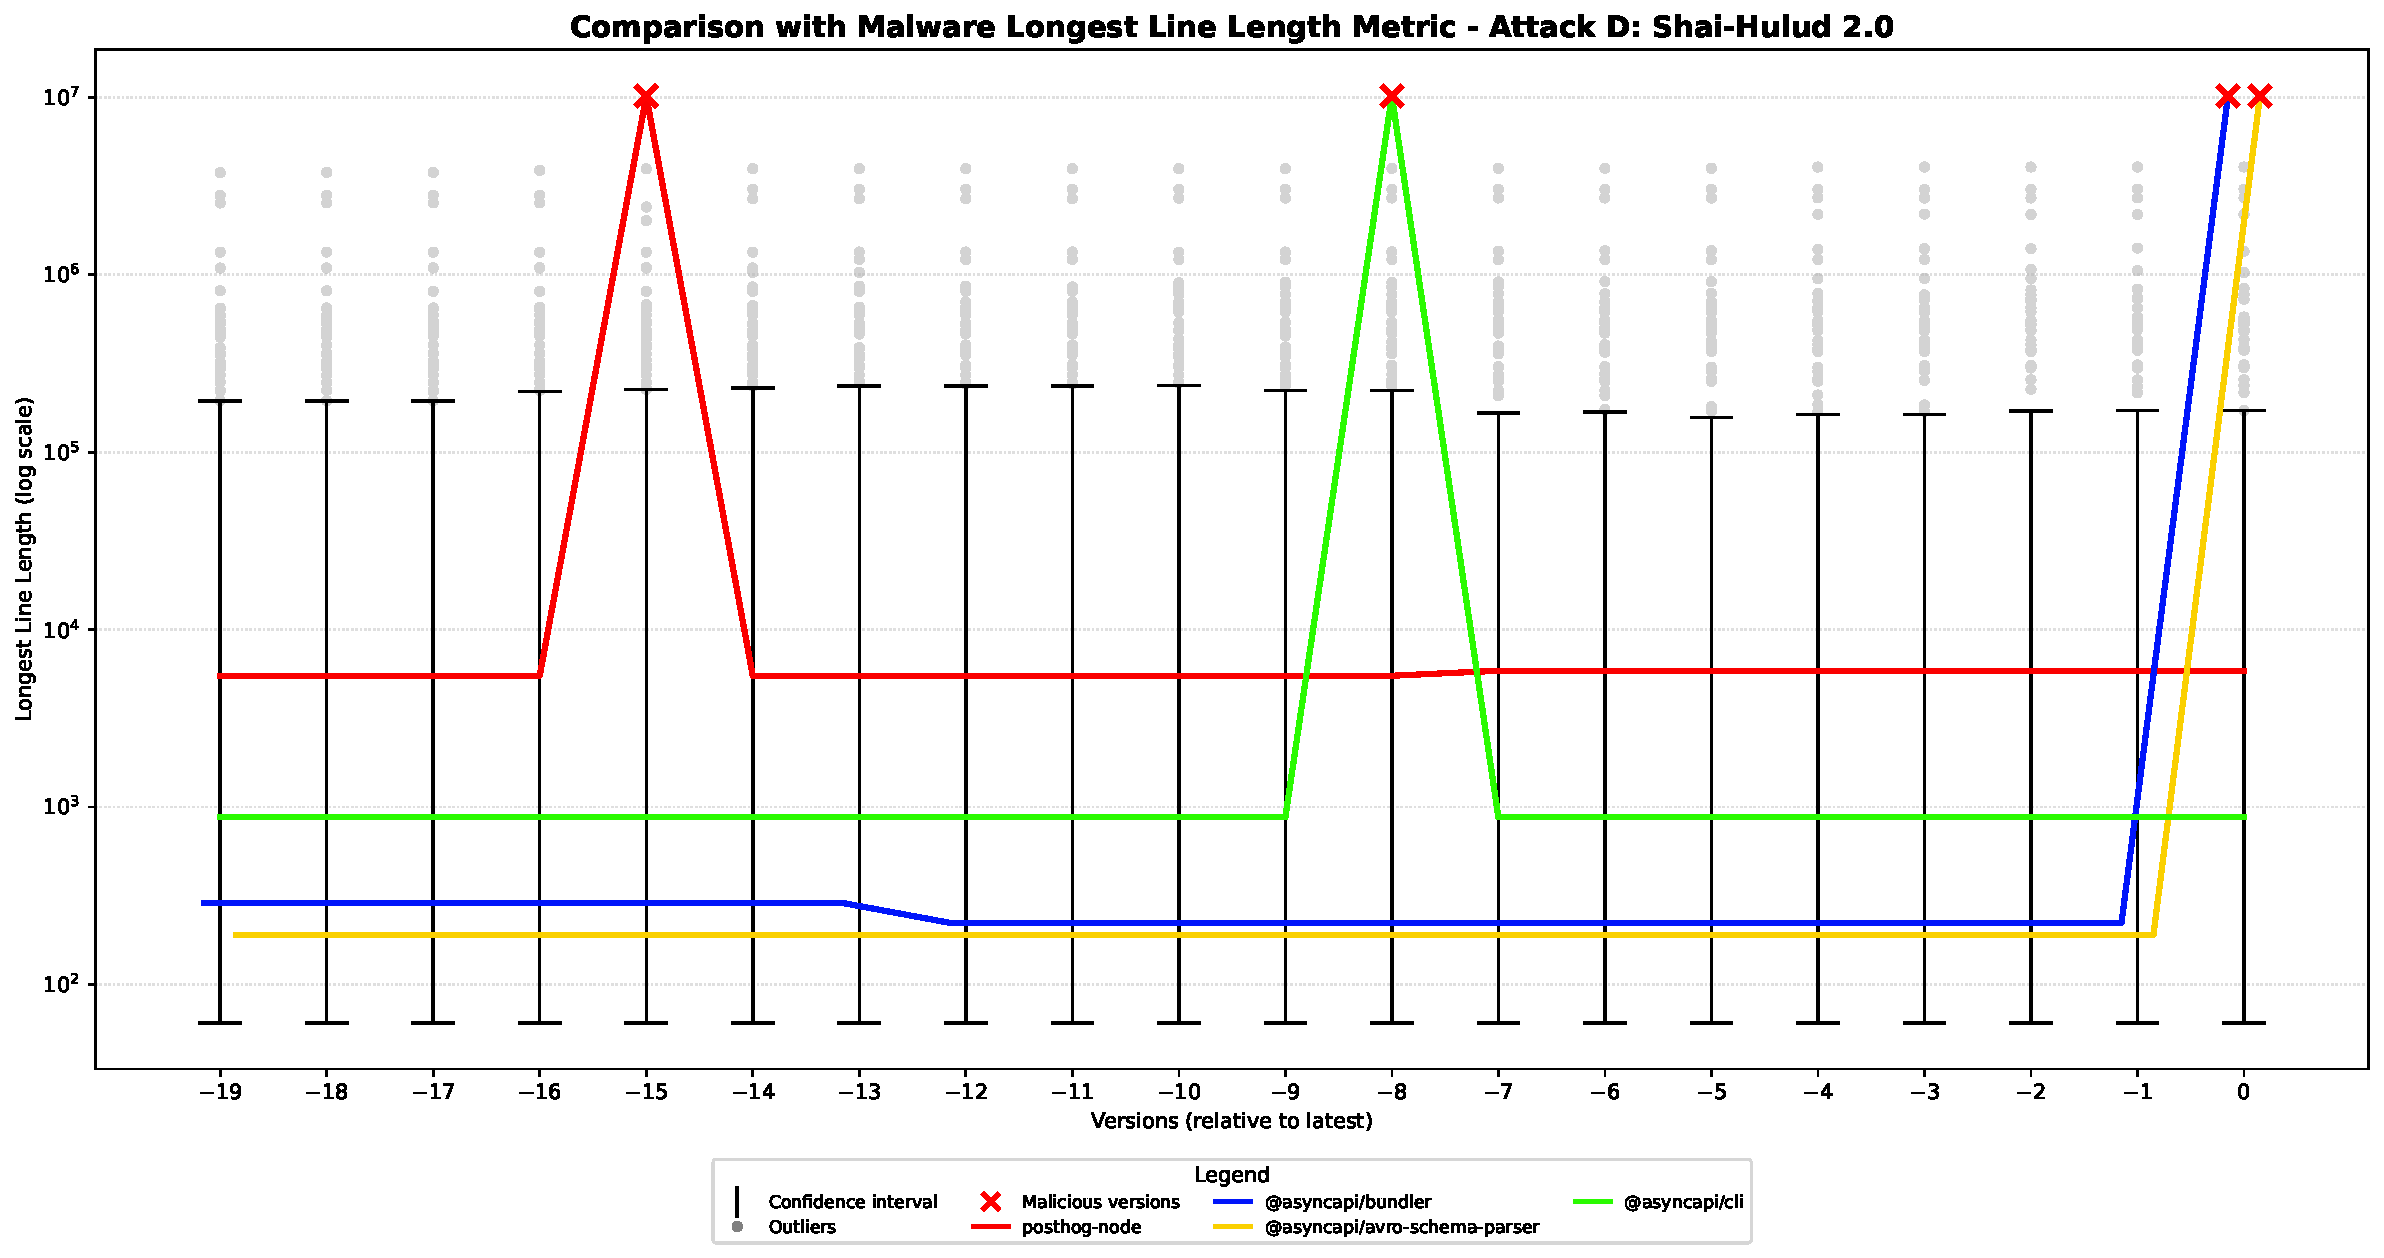
\includegraphics[width=0.90\textwidth]{metrics/LongestLineLength/LLL_plot2single_AttackD.pdf}
    \caption{Longest Line Length Metric: Malware Comparison for Attack~D.}
    \label{fig:fig2LLLAttackD}
\end{figure}